\documentclass[
]{elteikthesis}[2024/04/26]

\usepackage{lmodern}

\usepackage{geometry}
\geometry{margin=2.5cm}

\usepackage{pgfplots}
\pgfplotsset{compat=1.18}
\usetikzlibrary{arrows.meta,positioning}

\title{Ellenfél alapú támadások (FGSM, PGD) implementációja\\
konvolúciós neurális hálózatokhoz\\
interaktív tesztkörnyezetben}
\date{2026}

\author{Gabrity Gábor}
\degree{Programtervező Informatikus BSc}

\supervisor{Dr Varga Zsófia}
\affiliation{adjunktus}
\extsupervisor{Szabó András Miklós}
\extaffiliation{tanársegéd}

\university{Eötvös Loránd Tudományegyetem}
\faculty{Informatikai Kar}
\department{Térképtudományi és Geoinformatikai Intézet}
\city{Budapest}
\logo{elte_cimer_szines}

\addbibresource{Gabrity_Gabor_D9V09Z_Szakdolgozat.bib}
\ExecuteBibliographyOptions{maxnames=99}

\begin{document}

\documentlang{hungarian}

\maketitle

\newpage
\thispagestyle{empty}
\section*{Nyilatkozat}

Alulírott Gabrity Gábor, az Eötvös Loránd Tudományegyetem Informatikai Karának
hallgatója kijelentem, hogy ezt a szakdolgozatot saját magam készítettem, és abban csak a megadott
forrásokat használtam fel. Minden olyan részt, amelyet szó szerint vagy azonos tartalommal, de
átfogalmazva más forrásból átvettem, egyértelműen, a forrás megadásával megjelöltem.

A dolgozat bírálója által hátrányos értékeléssel nem járó exkluzív elektronikus hozzáférését a
benyújtástól számított két évig nem kérem.

\vspace{2cm}

Budapest, \today

\vspace{2cm}
\begin{flushright}
Gabrity Gábor s.k.\\
hallgató aláírása
\end{flushright}

\cleardoublepage

\tableofcontents
\cleardoublepage

\chapter*{Rövidítés- és jelölésjegyzék}
\addcontentsline{toc}{chapter}{Rövidítés- és jelölésjegyzék}
\cleardoublepage

\chapter{Bevezetés}

\section{Motiváció és a témaválasztás indoklása}

\section{A megoldandó feladat rövid, közérthető leírása}

\section{A dolgozat célja és hozzájárulásai}

\section{A dolgozat felépítése}

\chapter{Felhasználói dokumentáció}

\section{A megoldott probléma rövid megfogalmazása}

\section{A felhasznált módszerek rövid áttekintése}

\section{Rendszerkövetelmények}

\section{Telepítés és első indítás}

\section{A grafikus felhasználói felület bemutatása}

\section{Tipikus felhasználási forgatókönyvek}

\section{Hibaüzenetek és gyakori problémák}

\chapter{Fejlesztői dokumentáció}
Ebben a fejezetben a megvalósítandó szoftver célját és funkcióit formális, matematikai keretben definiálom, mivel a későbbi fejezetekben tárgyalt 
algoritmusok (FGSM, PGD) és a védekezési modul is ugyanerre a jelölésrendszerre épülnek majd. 
Először a probléma szereplőit, a modellt, a bemenetet és a hozzá tartozó címkét vezetem be, majd ezek segítségével pontosan megfogalmazom, mit 
is jelent az ellenfél alapú perturbáció. 
Ezután az itt bevezetett jelölésrendszerre épülve sorra bemutatom a két megvalósított támadási algoritmust (FGSM, PGD), a mögöttük álló tervezési 
döntéseket, a kapcsolódó munkákat, a védekezési stratégiákat, végül a szoftver architektúráját, a felhasznált technológiákat és az egyes 
komponensek megvalósítását. 

\section{A probléma részletes specifikációja}

\subsection{A modell, a bemenet és a címke}
Legyen adott egy $f_\theta$ neurális háló alapú osztályozó modell, melynek $x$ egy bemenete és $y$ annak helyes címkéje. 
Az $x$ bemenet ebben az esetben egy kép pixeleinek valamely három színű kódolása, vektoriális formában,
az $y$ pedig a kép helyes osztályának indexe (például $y=42$ az agámák ImageNet-1k osztályát reprezentálja). 
Amennyiben a képhez tartozó $y$ helyes címke nem ismert, úgy a modell által meghatározott legvalószínűbb címkét $\hat{y}$-nal jelöljük, és ezt 
használjuk referenciacímkeként. 

\subsection{A támadás célja}
Célunk az $x$ képre egy $x_{\mathrm{adv}}$ bemenet előállítása, mely az eredeti $x$-től szemmel csak alig látható perturbációban különbözik,
viszont a modell által adott $\hat{y}_{\mathrm{adv}} = \arg\max_i f_\theta(x_{\mathrm{adv}})_i$ predikció a referenciacímkétől eltér, vagy a 
klasszifikáció elbizonytalanodik. 

\subsection{Célzott és nem célzott mód}
Alapvetően két támadási módot különböztetünk meg, az ún. célzott és nem célzott módot. 
Nem célzott esetben a támadás célja minél jobban elbizonytalanítani a helyes osztályozást, tehát hogy agáma helyett bármi mást mutasson. 
Célzott módban azt szeretnénk, hogy egy kijelölt $y_{\mathrm{target}}$ osztály irányába változzon a képünk (pl.\ a komodói varánusz osztálya felé). 

\subsection{A white-box hozzáférési feltétel}
A támadás feltétele, hogy az $f_\theta$ modell gradienseihez és paramétereihez teljes hozzáférésünk legyen. 
Ezt white-box hozzáférésnek nevezzük az AI red teaming kontextusában. 

\subsection{A szoftver célja és beállítható paraméterei}
E szoftver célja a fenti ellenfél alapú támadó tesztkörnyezet szoftveres megvalósítása, különböző támadási algoritmusokkal (FGSM, PGD). 
A szoftver a PyTorch (torchvision) előtanított modelljeire épül, mely architektúra tetszőleges torchvision-modellel
bővíthető. Jelenleg kettő van integrálva (ResNet50, MobileNetV2). Beállíthatóak a futás paraméterei:
\begin{itemize}
  \item modell: ResNet50 vagy MobileNetV2, amelyen a támadást végrehajtjuk,
  \item $\epsilon$, mely meghatározza a perturbáció maximális mértékét, tehát azt, hogy egy pixelen legfeljebb mekkora
        változást tapasztalhatunk, azaz a változás felső határát,
  \item célosztály, $y_{\mathrm{target}}$, ha a mód célzott,
  \item iterációszám (PGD esetén hány lépésig engedjük futtatni az algoritmust).
\end{itemize}

\subsection{A felhasználói funkciók vázlatos áttekintése}

A fenti specifikációt a szoftver az alábbi, a felhasználó számára közvetlenül elérhető funkciókkal valósítja meg:
\begin{itemize}
  \item a fájlrendszerről kiválasztott képet legördülő menüből kiválasztott modellel klasszifikáljuk,
  \item támadási algoritmus és paraméterek meghatározásával perturbációt és ellenfél alapú képet generálunk,
  \item megjelenítjük az eredeti képet, a perturbációt és az ellenfél alapú képet, továbbá mindkét (eredeti és
        ellenfél alapú) képet osztályozzuk is,
  \item a védekezési modulban JPEG-tömörítést vagy más képfeldolgozási szűrőt alkalmazhatunk az ellenfél alapú perturbáció 
  hatásának utólagos csökkentésére vagy semlegesítésére,
  \item az eredeti és az ellenfél alapú kép PNG formátumban letölthető, a mentett képek pedig visszatölthetőek.
\end{itemize}

\section{Elméleti háttér és a használt fogalmak definíciója}

\subsection{Az osztályozó modell és a logitok}

Jelöljük $f_\theta(x) = z$-vel a modell outputjaként előállt valós számok tömbjét, ahol $z \in \mathbb{R}^C$ és $C$ az osztályok száma (ImageNet-1k esetén $C=1000$). 
Ezt logitvektornak is nevezzük, mely elnevezés a logisztikus regresszióból származik, ahol a $\mathrm{logit}(p) = \ln\frac{p}{1-p}$ függvény egy $p \in (0, 1)$ valószínűséget 
képez le a valós számegyenesre. 
A $z_i$ komponensek páronkénti különbsége éppen az $i$-edik és $j$-edik osztály esélyhányadosának logaritmusával egyezik meg, 
$z_i - z_j = \ln\frac{p_i}{p_j}$, innen származik az elnevezés.

\subsection{Valószínűségek és a modell predikciója}

Mivel a $z$ logitok önmagukban nem valószínűségek, a $\mathrm{softmax}$ függvénnyel alakítjuk át őket valószínűségi eloszlássá: 
\[
  p_i = \mathrm{softmax}(z)_i = \frac{e^{z_i}}{\sum_{j=1}^{C} e^{z_j}}, \qquad i = 1, \ldots, C.
\]
Tehát $p_i$ a modell szerint annak a valószínűsége, hogy $x$ az $i$-edik osztályba tartozik. 
A modell által meghatározott legvalószínűbb osztály indexét a legnagyobb valószínűségű komponens alapján kapjuk: 
\[
  \hat{y} = \arg\max_{i} p_i.
\]

\subsection{Veszteségfüggvény és bemeneti gradiens}

A $J(\theta, x, y)$ veszteségfüggvény a modell predikciója és a megadott helyes címke közötti eltérést méri. 
Esetünkben ez a keresztentrópia-veszteség 
\[
J(\theta, x, y) = -\log \frac{e^{z_y}}{\sum_{i=1}^{C} e^{z_i}},
\]
ahol $z = f_\theta(x)$ a logitvektor és $y$ a helyes osztály indexe. 
A veszteségfüggvény súlyok szerinti gradiense, $\nabla_\theta J(\theta, x, y)$, az a gradiensvektor, amelyet a hiba-visszaterjesztés (angolul \textit{backpropagation}) során a tanítás közben használunk a súlyok módosítására. 
Itt a gradiensszámítást egy további lépéssel a bemeneti rétegig visszük -- azaz a hiba-visszaterjesztés folyamatát a hálón teljesen végigvezetjük --, és megkapjuk a bemeneti vektorra vonatkozó érzékenységet, $\nabla_x J(\theta, x, y)$. 
Ez a mennyiség azt mutatja meg, hogy egy adott bemeneti pixel vagy jellemző változása milyen mértékben befolyásolja a veszteséget, ezért ennek a mennyiségnek központi szerepe 
lesz a későbbiekben bemutatott, ellenfél alapú példát generáló algoritmusok leírásában. 

\subsection{Perturbáció és normakorlát}

Az ellenfél alapú képek definíciójánál szokás a perturbáció nagyságát valamely $\ell_p$ normával jellemezni; ebben a dolgozatban a $\ell_\infty$ normát használjuk. 
Egy perturbált kép általában az
\[
  x_{\mathrm{adv}} = x + \delta
\]
formában írható le, ahol $\delta$ a zaj, vagyis a képpontokban okozott változás. 
A $\ell_\infty$ normát a 
\[
  \|v\|_\infty = \max_i |v_i|
\]
kifejezés definiálja, azaz a legnagyobb abszolút értékű komponens adja a norma értékét. 
A perturbáció nagyságát ezzel a normával korlátozzuk: 
\[
  \|\delta\|_\infty \leq \epsilon.
\]
Ez esetünkben nagyon kézenfekvő, mivel a bemeneti kép minden pixelén (minden $\delta_i$ komponensen) külön-külön korlátozza a megengedett változást. 

\section{Ellenfél alapú támadások áttekintése}
A mély neurális hálók, köztük a képfelismerő modellek is, különösen érzékenyek a bemeneti adatok kicsi, ám célzott módosításaira~\cite{goodfellow2015explaining}. 
Az ilyen módosításokat ellenfél alapú perturbációknak nevezzük. 
Ezeknek a támadásoknak két algoritmusát fogjuk itt átvenni, melyek a taxonómiában a korábban említett white-box támadások közé tartoznak. 
A következő fejezetekben egy egylépéses ellenfél alapú támadást mutatunk be (FGSM), utána erre építve egy többlépéses algoritmust (PGD). 

\subsection{FGSM (Fast Gradient Sign Method)}
Az FGSM algoritmust Goodfellow és szerzőtársai a Google-nél végzett kutatásaik alapján javasolták~\cite{goodfellow2015explaining}. 
Az előző fejezetben megjegyeztem, hogy a $\nabla_x J(\theta, x, y)$ veszteségfüggvény gradiense az input értékre való érzékenységet jelenti. 
Természetes ötlet, hogy a bemenetet a gradienssel ellentétes irányba mozdítsuk el, ami várhatóan növeli a veszteségfüggvény értékét, azaz rontja a 
helyes osztályra adott predikciót. 
Ehhez feltesszük, hogy a modell az $x$ pont kellően kis környezetében közelítőleg lineárisan viselkedik -- ez Goodfellow és társai linearitási 
elmélete, amely szerint a modern neurális hálók, részben a szakaszonként lineáris aktivációk (pl.\ ReLU) miatt, lokálisan jól közelíthetők egy 
lineáris függvénnyel, még ha globálisan erősen nemlineárisak is~\cite{goodfellow2015explaining}. 
Az FGSM algoritmusban az elmozdítást egyszerűen csak az előjel-függvény ($\mathrm{sign}$) $\epsilon$-szorosával tesszük meg, tehát nem vesszük 
figyelembe a gradiens nagysága által adott érzékenységet, csak az irányát. 
Ily módon az $\epsilon \cdot \mathrm{sign}(\cdot)$ minden egyes $x_i$ komponensre kihasználja a teljes $\epsilon$ költségvetésünket. 
Tehát az FGSM ellenfél alapú példát a következő módon kapjuk meg: 
\[
  x_{\mathrm{adv}} = x + \epsilon \cdot \mathrm{sign}\big(\nabla_x J(\theta, x, y)\big).
\]

\subsubsection{Célzott változat}
Az alapváltozat a megadott helyes osztály veszteségét igyekszik maximalizálni, tehát minél inkább mást mutasson, mint ami a képen van. 
A célzott változatnál egy $y_{\mathrm{target}}$ célosztályt adunk meg, és azt szeretnénk, hogy a modell ebbe az osztályba sorolja az ellenfél alapú képet. 
\[
  x_{\mathrm{adv}} = x - \epsilon \cdot \mathrm{sign}\big(\nabla_x J(\theta, x, y_{\mathrm{target}})\big).
\]
Tehát a képlet csak annyiban változik, hogy távolodás helyett az $y_{\mathrm{target}}$-hoz tartozó veszteség minimuma felé közeledni szeretnénk, és $y$ helyett $y_{\mathrm{target}}$-ot használjuk. 

\subsubsection{Előnyök és korlátok}
Mivel a gradienst a tanításban is használt hiba-visszaterjesztés segítségével hatékonyan tudjuk kiszámolni, ezért a támadás gyors. 
Hátránya, hogy csak egyetlen, durva lépést tesz a megfelelő irányba, ezért -- főleg az iteratív módszerekhez, például a PGD-hez képest -- 
kevésbé hatékonyan képes megtéveszteni az osztályozót. 

\subsection{PGD (Projected Gradient Descent)}
Ezt a módszert Madry és társai vezették be~\cite{madry2018towards}, és lényegében az FGSM egylépéses ötletének iteratív általánosítása. 
Nem egyetlen nagy lépést teszünk a gradiens előjele irányába, hanem ugyanabba az irányba több, kisebb lépést hajtunk végre egymás után. 
A motiváció emögött az, hogy az FGSM linearitási feltevése csak $x$ kellően kis környezetében állja meg a helyét, ezért előnyösebb, ha $T$ darab 
kisebb, $\alpha$ nagyságú lépéssel dolgozunk, és a gradienst minden lépésben újraszámoljuk. 
Legyen $S = \{\delta : \|\delta\|_\infty \leq \epsilon\}$ a megengedett perturbációk halmaza; ekkor $x+S$ adja meg az $x$ körüli, $\epsilon$ 
sugarú gömbbe eső, engedélyezett bemenetek halmazát. 
($\ell_\infty$ norma esetén ez geometriailag valójában egy kocka, de általános $\ell_p$ értelemben vett gömbként hivatkozunk rá.) 
Mivel az iteráció túlléphet $x+S$ korlátján, az algoritmus minden lépés után egy projekcióval visszavetíti az eredményt erre a halmazra. 
Ez FGSM esetén a $\mathrm{sign}$ függvény miatt automatikusan teljesült, itt viszont $T$ és $\alpha$ megválasztásától függően külön biztosítani kell. 
Az algoritmus formális definíciója tehát 
\[
  x^{t+1} = \Pi_{x+S}\big(x^t + \alpha \cdot \mathrm{sign}(\nabla_x J(\theta, x^t, y))\big), \qquad x^0 = x,
\]
ahol $\Pi_{x+S}$ az $x+S$ halmazra való projekció.

\subsubsection{Célzott változat}
Az FGSM-hez hasonlóan itt is definiálunk egy célzott változatot, amely az ottanival analóg módon adható meg: 
\[
  x^{t+1} = \Pi_{x+S}\big(x^t - \alpha \cdot \mathrm{sign}(\nabla_x J(\theta, x^t, y_{\mathrm{target}}))\big).
\]

\subsubsection{Véletlen kiindulási pont}
Madry és társai kísérletileg mutatták meg, hogy a veszteségfelszín lokális maximumai jól koncentráltak, így egy véletlen kezdőpontból indított PGD 
is megbízhatóan jó megoldást talál~\cite{madry2018towards} (a jelenség hátterét a \ref{sec:saddle-point-landscape}. alfejezet tárgyalja részletesen). 
Ennek a modellek robusztusságának tesztelésében is van szerepe: mivel a veszteségfelszínnek több, egymástól távol eső lokális maximuma is lehet, egy 
fix (pl.\ magából $x$-ből induló) kezdőpont esetén a szerencsének nagy szerepe lehetne, és az eredmény nem feltétlenül mutatná a modell valódi 
sebezhetőségét. 
Ezért a véletlen kezdőpontot az $\epsilon$ sugarú gömbben egyenletes eloszlással választjuk meg: 
\[
  x^0 = \Pi_{x+S}(x + \eta), \qquad \eta \sim \mathcal{U}(-\epsilon, \epsilon)^d.
\]

\subsubsection{Az $\alpha$ és $T$ paraméterek megválasztása}
A PGD viselkedését az $\epsilon$ perturbációs korláton felül két további paraméter határozza meg. 
$T$ az iterációk számát jelöli, ez adja meg az algoritmus számítási költségét, ugyanakkor több iteráció jellemzően erősebb támadást eredményez. 
Az $\alpha$ lépésnagyságot úgy kell megválasztani, hogy túl kicsi érték esetén lassú a konvergencia, túl nagy érték esetén pedig instabilitáshoz 
vezethet. 
Tipikus választás: $\alpha = \epsilon / T$ vagy $\alpha = 2{,}5 \cdot \epsilon / T$~\cite{madry2018towards}.

\subsubsection{Előnyök és korlátok}
A PGD az FGSM-nél lényegesen erősebb támadásokat képes generálni, mivel több kis lépésben közelíti a lokális optimumot. 
A véletlen kezdőponttal kombinálva különösen hatékony a robusztusság kiértékelésében. 
Hátránya, hogy $T$-szer annyi gradiens-számítást igényel, mint az FGSM, így nagyobb a számítási költsége. 

\section{Továbbmutató elméleti vonatkozások}
Ebben a fejezetben azokat az elméleti vonatkozásokat foglalom össze, amelyek nem képezik szigorúan a dolgozatban megvalósított szoftver részét, ám fontos 
kiegészítői annak.

\subsection{Linearitás}
\label{sec:linearity}
Goodfellow és társai az ellenfél alapú példák létezésére nem a neurális hálók feltételezett, extrém nemlinearitásán vagy túltanulásán alapuló 
magyarázatot adnak. 
Ehelyett ennek éppen az ellenkezőjét állítják. 
Szerintük a jelenség hátterében a modern modellek meglepően lineáris viselkedése 
áll~\cite{goodfellow2015explaining}. 

A legegyszerűbb esetben tekintsünk egy lineáris klasszifikátort $w$ súlyvektorral, tehát egy egyrétegű modellt. Vizsgáljuk az ellenfél alapú
 $\tilde{x} = x + \eta$ bemenet aktivációját. 
\[
  w^\top \tilde{x} = w^\top x + w^\top \eta.
\]
A $\|\eta\|_\infty \leq \epsilon$ korlát mellett a $w^\top \eta$ növekmény akkor maximális, ha $\eta = \epsilon \cdot \mathrm{sign}(w)$. 
Ez pontosan az FGSM képletének lineáris modellre vonatkozó speciális esete. 
Ha $w$ dimenziója $n$, és egy komponensének átlagos nagysága $m$, akkor az aktiváció növekménye $\epsilon m n$ nagyságrendű. 
Mivel $\|\eta\|_\infty$ maga nem nő a dimenziószámmal, az általa okozott aktivációváltozás viszont lineárisan nő $n$-nel, ezért elég nagy 
dimenziójú bemenet esetén sok, egyenként elhanyagolhatóan kicsi (a pixelek $8$ bites kódolási pontosságánál is kisebb) elmozdítás összegződve 
tetszőlegesen nagy kimeneti változást okozhat. 
Ez azt mutatja, hogy már egy egyszerű lineáris modellnek is lehetnek ellenfél alapú példái, ha a bemenete elég nagy dimenziójú. 

Goodfellow és társai szerint a modern neurális hálók (pl.\ ReLU, maxout, LSTM) tudatosan lineáris viselkedésre vannak 
tervezve, mivel ez megkönnyíti az optimalizálásukat.
Emiatt ezek a hálók, megfogalmazásuk szerint "túl lineárisak" ahhoz, hogy ellenálljanak egy lineáris ellenfél alapú perturbációnak. 
Ez a megfigyelés adja a korábban bemutatott FGSM elméleti alapját. 

\subsection{Transzferálhatóság}
Az ellenfél alapú perturbációk egyik legfontosabb tulajdonsága a transzferálhatóság, ami azt jelenti, hogy egy adott $f_\theta$ modellre 
kiszámított $x_{\mathrm{adv}}$ sokszor egy másik, eltérő architektúrájú, más inicializálású, vagy akár más adathalmazon tanított modellt is 
megtéveszthet.
Tehát a megtévesztés úgy is megtörténhet, hogy a perturbációt nem az ő gradienseiből számoltuk, azaz lehetővé teszi a black-box támadásokat. 
Ehhez elég egy hasonló feladatra tanított modellen white-box módon (pl.\ FGSM vagy PGD segítségével) előállítani a perturbációt, majd azt a 
célmodellen felhasználni. 
Goodfellow és társai a jelenség magyarázatát is a \ref{sec:linearity}. alfejezetben bemutatott linearitási hipotézisre vezetik vissza. 
Szerintük a különböző architektúrájú modellek ugyanazon adathalmazon hasonló, közelítőleg lineáris döntési határt tanulnak meg, ezért egy adott 
modellre számolt perturbáció a hasonló döntési határ miatt más modelleket is megtéveszt~\cite{goodfellow2015explaining}. 

Goodfellow és társai kísérletileg igazolták a transzferálhatóságot. 
Az FGSM-mel az eredeti modellre generált ellenfél alapú példák 19,6\%-os hibaarányt okoztak egy másik, ellenfél alapú tanítással robusztusabbá 
tett modellen, míg az utóbbi modellre generált példák 40,9\%-os hibaarányt okoztak az eredetin. 
Ezek szerint a robusztusabb modellről származó perturbációk erősebbnek bizonyultak a transzfer irányban is~\cite{goodfellow2015explaining}. 

Madry és társai ezt a jelenséget rendszerezettebben, több modellpár és mindkét vizsgált algoritmus (FGSM, PGD) összehasonlításával vizsgálták, és 
két fő tendenciát azonosítottak. 
Minél erősebb az a támadó (adversary), amellyel a forrásmodellt tanították, illetve minél nagyobb a modell 
kapacitása, annál kevésbé transzferálhatóak a rá generált ellenfél alapú példák más modellekre~\cite{madry2018towards}. 
Ennek oka, hogy a nagyobb kapacitású, erősebb támadó ellen (pl.\ PGD-vel) tanított modellek veszteségfelszíne kevésbé korrelál a többi modellével, 
így a rájuk kiszámított gradiensirány egyre kevésbé lesz általánosan érvényes. 


\subsection{A nyeregpont (saddle point) optimalizálási keret és a lokális maximumok koncentrációja}
\label{sec:saddle-point-landscape}
Madry és társai az ellenfél alapú robusztusságot a robusztus optimalizálás nyelvén, egy úgynevezett nyeregpont- (angolul \textit{saddle point}, 
más néven min-max) feladatként fogalmazzák meg~\cite{madry2018towards}: 
\[
  \min_\theta \; \rho(\theta), \qquad \rho(\theta) = \mathbb{E}_{(x,y)\sim \mathcal{D}} \Big[ \max_{\delta \in S} J(\theta, x+\delta, y) \Big],
\]
ahol $S = \{\delta : \|\delta\|_\infty \leq \epsilon\}$ a korábban bevezetett, megengedett perturbációk halmaza. 
A belső maximalizálási feladat a támadás problémáját írja le. 
Ez az adott $\theta$ paraméterű modellhez a veszteséget maximalizáló $\delta$ perturbáció megtalálását jelenti. 
A külső minimalizálási feladat a védekezés problémája, tehát olyan $\theta$ paraméterek keresése, amelyek mellett a belső maximalizálás által adott 
a legrosszabb esetű veszteség is minél kisebb. 
Ez a maximum minimalizálás pontosan az ellenfél alapú tanítás célja. 

Mivel a belső feladat egy erősen nem konkáv függvény maximalizálása, elsőre nem várnánk, hogy megbízhatóan megoldható. 
Az ilyen feladatoknak sokszor egymástól távol eső lokális maximumai lehetnek, és nincs rá garancia, hogy egy gradiens alapú módszer 
a globális maximum közelébe jut. 
Madry és társai ezt a kérdést kísérletileg vizsgálták. 
Ebben sok, független, véletlenszerűen választott kezdőpontból indítottak PGD-t ugyanazon $x$ bemenet $\epsilon$ sugarú gömbön belül, és 
a talált lokális maximumok tulajdonságait figyelték~\cite{madry2018towards}. 
Azt találták, hogy bár a talált lokális maximumok ténylegesen különbözőek, az általuk elért veszteségértékek meglepően szűk sávban 
koncentrálódnak, extrém kiugró érték nélkül. 
A veszteség emellett viszonylag kevés iteráció után platóra ér, tehát a PGD gyorsan konvergál egy, a globálishoz közeli értékhez, függetlenül a 
konkrét kezdőponttól. 
Ez a jelenség rokon azzal a tapasztalati megfigyeléssel, hogy a neurális hálók tanítása azért működik jól annak ellenére, hogy a 
veszteségfelszín is sok lokális minimumot tartalmaz. 
Ezek a lokális minimumok ugyanis szintén hasonló értékűek egymáshoz. 
Ugyanez a regularitás jelentkezik itt a bemeneti perturbáció szerinti belső maximalizálásra vonatkozóan is. 
Ez azt mutatja, hogy a belső feladat a nem konkávsága ellenére is jól kezelhető, ,,szelíd'' szerkezetű (\ref{fig:loss-landscape-local-maxima}. ábra). 

\begin{figure}[htb]
\centering
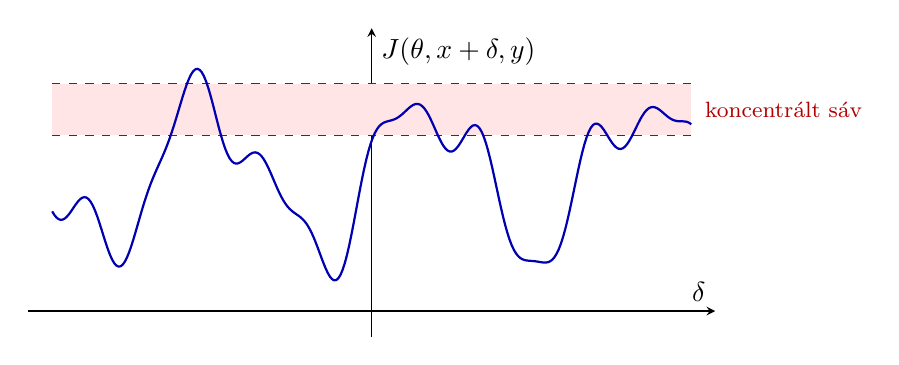
\begin{tikzpicture}
\begin{axis}[
    width=0.85\textwidth,
    height=5.5cm,
    domain=-4:4,
    samples=300,
    axis lines=middle,
    xlabel={$\delta$},
    ylabel={$J(\theta, x+\delta, y)$},
    xtick=\empty,
    ytick=\empty,
    ymin=-0.3, ymax=3.3,
    xmin=-4.3, xmax=4.3,
    clip=false,
]
\fill[red!10] (axis cs:-4,2.05) rectangle (axis cs:4,2.65);
\draw[dashed, red!70!black] (axis cs:-4,2.05) -- (axis cs:4,2.05);
\draw[dashed, red!70!black] (axis cs:-4,2.65) -- (axis cs:4,2.65);
\addplot[thick, blue!70!black] {1.6 + 0.85*sin(deg(2.3*x)) + 0.35*sin(deg(5*x+0.7)) + 0.18*sin(deg(9*x+2))};
\node[red!70!black, anchor=west, font=\footnotesize] at (axis cs:4.05,2.35) {koncentrált sáv};
\end{axis}
\end{tikzpicture}
\caption{Sematikus ábra a veszteségfüggvény $\delta$ perturbáció szerinti. Sok, egymástól távol eső lokális 
maximum létezik, ezek értékei egy szűk sávban koncentrálódnak.}
\label{fig:loss-landscape-local-maxima}
\end{figure}

Ez a felismerés adja a PGD elméleti indoklását mint a legrosszabb esetű, kizárólag elsőrendű (gradiens-) információt felhasználó ellenfelek közül 
a legerősebbet, az ún.\ ,,univerzális első rendű ellenfelet''. 
Ez azért van, mert a kezdőponttól függetlenül megbízhatóan hasonlóan jó, a globálishoz közeli megoldást talál. 


\subsection{Ellenfél alapú tanítás}
A \ref{sec:saddle-point-landscape}. alfejezetben bemutatott nyeregpont-feladat külső minimalizálási része pontosan az ellenfél alapú tanítás 
elméleti megfogalmazása. 
Ez azon $\theta$ paraméterek keresését jelenti, amelyek mellett a belső maximalizálás által adott, legrosszabb esetű veszteség is 
minél kisebb. 
Ennek gyakorlati megvalósításához a tiszta $x$ kép mellett a hozzá tartozó $x_{\mathrm{adv}}$ ellenfél alapú képet is bevonjuk a 
veszteségfüggvénybe, és a modell paramétereit az így kapott kombinált célfüggvényre optimalizáljuk. 

Goodfellow és társai az FGSM-mel előállított $x_{\mathrm{adv}}$ perturbációra a következő kombinált veszteségfüggvényt 
javasolták~\cite{goodfellow2015explaining}: 
\[
\tilde{J}(\theta, x, y) = \lambda \, J(\theta, x, y) + (1-\lambda)\, J(\theta, x_{\mathrm{adv}}, y), \qquad \lambda = 0{,}5.
\]
Az új veszteségfüggvény tehát a tiszta és az ellenfél alapú minta hibáját egyaránt bünteti, méghozzá úgy, hogy $x_{\mathrm{adv}}$-ot minden tanítási lépésben a 
modell aktuális $\theta$ paramétereivel újraszámolják. 
Így tehát a modell a tanítás során folyamatosan fejlődik, és az aktuális állapota által generált ellenfél alapú példákon tanul tovább dinamikusan, nem pedig 
egy előre legyártott, statikus ellenfél alapú halmazon. 
Kísérleteik megmutatták, hogy ez egy hatékony módszer. 
Az FGSM-mel előállított ellenfél alapú példákon mért hibaarány 89,4\%-ról 17,9\%-ra csökkent. 

Madry és társai megmutatták, hogy PGD-vel is alkalmazható az ellenfél alapú tanítás, és erősebb védekezést eredményez~\cite{madry2018towards}. 
Itt azonban a tiszta és ellenfél alapú veszteséget kombináló FGSM-formulával ellentétben nincs szó keverésről. 
A tanítás során a tiszta $x$ kép helyett kizárólag a hozzá tartozó, PGD-vel előállított $x_{\mathrm{adv}}$-on számolják a veszteséget, tehát a modell csak az ellenfél alapú bemeneteken tanul. 
Mivel a PGD erősebb támadás, mint az FGSM, az ellene edzett modell a gyengébb, egylépéses támadásokkal szemben is ellenállóbb marad, míg a fordítottja nem 
feltétlenül igaz. 

\subsection{Madry és társai következtetései}
Madry és társai eredményei azt igazolják, hogy a mély neurális hálók ellenálló képessége az ellenfél alapú támadásokkal szemben megbízhatóan 
növelhető. 
Kísérleti eredményeik alapján megbízható ellenfél alapú tanítási módszerek tervezhetők~\cite{madry2018towards}. 
Ennek egyik kulcsfontosságú alapja a fenti felismerés, miszerint a PGD adja az univerzális első rendű ellenfelet. 
Mindezek alapján a szerzők úgy vélik, hogy az ellenfél alapú támadásokkal szemben robusztus mély tanulási modellek a jelenlegi eszközökkel is 
elérhetőek. 
Kísérleti eredményeik ugyanakkor azt is megmutatták, hogy ez a robusztusság adathalmaz-függő. 
MNIST adathalmazon (szürkeárnyalatos kézzel írott számjegyek) a hálóik igen robusztusnak bizonyultak, és nagy pontosságukat erős 
$\ell_\infty$-korlátos ellenfelek és nagy perturbációk esetén is megtartották. 
A bonyolultabb CIFAR10 adathalmazon (színes, természetes fényképek 10 kategóiában) a kísérleteik ezt a szintet még nem érték el. 
Az eredményeik azonban itt is jelentős javulást mutattak a robusztusságban.

\section{Kapcsolódó munkák és további támadási módszerek}

\subsection{Optimalizáció-alapú korai módszerek}
Az ellenfél alapú perturbáció fogalmának első dokumentált megjelenése Szegedy és társai nevéhez fűződik~\cite{szegedy2014intriguing}. 
Módszerük a támadást egy explicit optimalizálási feladatként fogalmazza meg. 
A cél egy olyan, $\ell_2$ normában minimális $\delta$ perturbáció megtalálása, amely mellett a modell predikciója egy előre megadott $y_{\mathrm{target}}$ 
célosztályra változik.
\[
  \min_{\delta} \|\delta\|_2 \qquad \text{úgy, hogy} \qquad \arg\max_i f_\theta(x+\delta)_i = y_{\mathrm{target}}, \quad x+\delta \in [0,1]^n.
\]
Ezt a feltételes feladatot Szegedy és társai a korlátozott memóriaigényű Broyden--Fletcher--Goldfarb--Shanno módszer (L-BFGS) egy dobozkorlátos 
változatával közelítették, amely egy kvázi-Newton típusú numerikus optimalizálási technika. 
Kísérleteikben mutatták meg először a korábban tárgyalt transzferálhatóságot, mint a neurális hálók egyik tulajdonságát. 

Ez a korai módszer white-box hozzáférést és gradiens alapú optimalizálást igényelt, hasonlóan a korábban bemutatott FGSM-hez és PGD-hez. 
A lényegi különbség az, hogy itt egy konvergenciáig futó optimalizálási feladatot kell megoldani. 
Ez számításigényesebb, mint az FGSM egyetlen lépése vagy a PGD rögzített iterációszáma. 
Ez a számítási költség adta a motivációt Goodfellow és társai számára egy hatékonyabb, egylépéses módszer kidolgozásához, amit a korábban 
bemutatott FGSM-ként ismerünk~\cite{goodfellow2015explaining}. 
A NIST 2025-ös, ellenfél alapú gépi tanulásról szóló átfogó jelentése szerint jól dokumentált történeti fejlődési láncot alkot a szakirodalomban 
az optimalizáció-alapú korai módszerektől (Szegedy és társai) az FGSM-en és Kurakin és társai iteratív FGSM-változatán át egészen a 
PGD-ig~\cite{nist2025aml}. 

\subsection{Univerzális perturbációk}
Az eddigi módszerek mindegyike digitális támadás, a $\delta$ perturbációt egyetlen konkrét $x$ bemenetre 
számolja ki, tehát minden új képhez elvégzi a gradiensszámítást. 
Moosavi-Dezfooli és társai ezzel szemben megmutatták, hogy képek egy adott halmazára létezik egyetlen, kép-független 
(\textit{image-agnostic}) perturbációs vektor is, amely a képek jelentős részére alkalmazva önmagában téves osztályozást eredményez~\cite{moosavidezfooli2017universal}. 
Az ilyen perturbációt univerzálisnak nevezik. 
Formálisan, ha $\mu$ a bemeneti képek eloszlása és $\hat{y}(x)$ a modell által adott predikció, akkor egy $v$ perturbációs vektort keresnek, 
amelyre 
\[
  \|v\|_p \leq \xi \qquad \text{és} \qquad \Pr_{x\sim\mu}\big[\hat{y}(x+v) \neq \hat{y}(x)\big] \geq 1-\delta,
\]
ahol $\xi$ a megengedett perturbáció nagyságát korlátozza, $\delta$ pedig a kívánt tévesztési arányt (\textit{fooling rate}) határozza meg. 

A szerzők egy iteratív algoritmust javasolnak a $v$ vektor előállítására, amely a tanítóképek egy $X$ részhalmazán dolgozik, és képenként 
addig módosítja a már felhalmozott perturbációt, amíg az adott kép át nem kerül a döntési határ túloldalára, minden lépés után visszavetítve az 
eredményt a $\xi$ sugarú $\ell_p$ gömbre. 
Az eljárás lényegi újdonsága, hogy a $v$ vektort elég egyszer kiszámítani egy viszonylag kis képhalmazon, ezt követően új bemenetekre való 
alkalmazásához elegendő a vektor egyszerű hozzáadása, gradiensszámítás vagy újabb optimalizálás nélkül. 

Kísérleteik szerint egy, néhány ezer (akár csak néhány száz) képen számolt univerzális perturbáció a validációs halmaz eddig nem látott 
képeinek túlnyomó részén, esetenként 80--90 százalék felett is, téves osztályozást eredményez, annak ellenére, hogy szemmel alig észrevehető. 
%Emellett a korábban bemutatott transzferálhatóság egy erősebb változatát is mutatja: egy adott architektúrára (például VGG-19-re) számolt 
%perturbáció más, jelentősen eltérő architektúrájú hálókon (GoogLeNet, ResNet) is számottevő tévesztési arányt ér el, tehát nemcsak a képek, 
%hanem a modellarchitektúrák között is általánosít, ami a szerzők szerint a döntési határok közötti geometriai hasonlóságra, és így a korábban 
%bemutatott linearitási hipotézisre vezethető vissza.

\subsection{Fizikailag megvalósítható támadások}
Az eddig tárgyalt módszerek digitális támadások, a perturbációt közvetlenül a modellnek átadott kép pixeleire számolják ki. 
A fizikailag megvalósítható támadások ezzel szemben olyan perturbációkat állítanak elő, amelyek a valós környezetben is kivitelezhetőek.

Sharif és társai egy nyomtatott szemüvegkeret mintázatát optimalizálták úgy, hogy azt viselve a támadó elkerülje a felismerést, vagy más 
személynek adja ki magát~\cite{sharif2016accessorize}. 
A perturbációt egy gradiens alapú optimalizálással, egy simasági (\textit{total variation}) megszorítással kiegészítve állították elő, amely 
biztosítja, hogy a mintázat nyomtatható és kamerával visszafényképezhető maradjon. 
Ezt a nyomtatott szemüveget felvéve a résztvevők az esetek nagy részében sikeresen elkerülték a felismerést, egyes célszemélyeknél a megszemélyesítés is 
jelentős arányban sikerült. 

Eykholt és társai egy hasonló elven működő, közlekedési táblák elleni támadást dolgoztak ki, Robust Physical Perturbations (RP2) néven~\cite{eykholt2018robust}. 
A perturbációt nem egy kép pixeleire, hanem a fizikai környezet változatosságát (eltolás, elforgatás, megvilágítás, távolság) modellező 
eloszlásra optimalizálják, így az a különböző körülmények között készült felvételeken is robusztus marad. 
Fekete-fehér matricák formájában egy valódi Stop táblára helyezett ilyen formájú perturbáció tábla típusát tévesen azonosította be. 
Laboratóriumi teszteken teljes, a mozgó járműből rögzített videón pedig igen magas sikerességi arányt értek ezzel el.  

Chen és társai a fizikailag megvalósítható támadások körét objektumdetektorokra terjesztették ki, ShapeShifter néven~\cite{chen2018shapeshifter}. 
Ez nehezebb feladat, mert a detektornak egyszerre több, különböző méretű régióban (\textit{bounding box}) kell tévesen felismernie az objektumot. 
A szerzők az úgynevezett várható érték a transzformáció felett (\textit{Expectation over Transformation}) technikát adaptálták erre a feladatra, 
és az így létrehozott, nyomtatott Stop táblák a Faster R-CNN detektort a valóságban, különböző távolságokból és szögekből felvéve is 
következetesen megtévesztették. 

A közös tanulság, hogy itt a robusztusságot nem elegendő egyetlen rögzített bemenetre biztosítani, a perturbációnak a fizikai körülmények 
(nézőpont, távolság, megvilágítás, kamera- és nyomtatási torzítás) teljes változatosságával szemben is meg kell maradnia, ami a támadási 
felületet a valós, fizikai környezetbe is kiterjeszti, és az önvezető járművek vagy beléptető rendszerek biztonságát közvetlenül érinti. 

\section{Védekezési stratégiák áttekintése}
Most pár egyszerűbb védekezési stratégiát nézünk, amelyek a bemeneti képet alakítják át pont a klasszifikáció előtt, remélve, hogy az átalakítás 
eltávolítja, de legalább csökkenti a perturbáció hatását. 
A szoftver védekezési moduljában két ilyen módszert, a JPEG-tömörítést és a Gauss-elmosást nézzük itt át. 
Közös bennük, hogy egyszerűek, nem igényelnek újratanítást vagy hozzáférést a modell gradienseihez, viszont csak kisebb perturbációjú támadások 
ellen biztosítanak védelmet. 
Céljuk elsősorban szemléltető, illetve a perturbáció utólagos csökkentésének demonstrálására szolgáló eszközként tekintendő, 
nem pedig egy megbízható, önmagában elégséges védelmi mechanizmusként. 

\subsection{A JPEG-tömörítés mint védekezés}
Dziugaite és társai kifejezetten a JPEG-tömörítés ellenfél alapú perturbációkra gyakorolt hatását vizsgálták~\cite{dziugaite2016jpeg}. 
Hipotézisük szerint a természetes képek egy alacsony dimenziós altérben, az adataltérben helyezkednek el, egy ellenfél alapú perturbáció 
viszont jellemzően kimozdítja a képet ebből az altérből. 
Mivel a képosztályozási adathalmazok szinte kivétel nélkül JPEG formátumú képekből állnak, egy újratömörítés a perturbált képet visszavetítheti egy, 
az adataltérnél tágabb, de azt magába foglaló altérbe, az úgynevezett JPEG-altérbe. 
Feltételezésük szerint ez az újratömörítés legalábbis részben visszaállíthatja a klasszifikáció helyességét. 

Eredményeik szerint kis magnitúdójú perturbáció ($\epsilon=1/255$) esetén a JPEG-tömörítés jelentős mértékben, bár nem teljesen, visszaállította a 
klasszifikációs pontosságot. 
Nagyobb magnitúdójú perturbációk ($\epsilon=5/255$ és $\epsilon=10/255$) esetén az újratömörítés hatása elenyésző volt, a pontosság nem tért vissza a 
tiszta képekre jellemző szintre. 
Ebből azt a következtetést vonták le, hogy a JPEG-tömörítés önmagában nem nyújt megbízható védelmet az ellenfél alapú perturbációkkal szemben, 
hatékonysága erősen függ a perturbáció nagyságától. 

\subsection{A Gauss-elmosás mint védekezés}
A Gauss-elmosás egy szűrő, aminél minden pixel értéket a szomszédos pixelek átlagaként állítjuk elő, azaz letompítjuk azt. 
Dziugaite és társai megemlítik, hogy Kurakin és társai egy korábbi munkájukban a JPEG-tömörítés mellett vizsgálták a Gauss-elmosást, valamint 
a fényerő és a kontraszt módosítását is, vagy akár a fizikai világban (nyomtatás és újrafényképezés) átalakított módszereket, mint lehetséges 
védekezési módszereket~\cite{dziugaite2016jpeg}. 
Ez a hivatkozott vizsgálat azt találta, hogy az FGSM-perturbációk viszonylag ellenállóak az ilyen képtranszformációkkal szemben. 

\section{A rendszer architektúrája}
A szoftver egyetlen, önálló asztali alkalmazásként fut, hálózati backend nélkül, ezért architektúrája nem a megszokott kliens--szerver 
felosztást követi, hanem a felelősségek szerint különül el belső rétegekre. 
A rétegek a következők, a belépési ponttól a legmélyebb logikáig haladva: 

\begin{itemize}
  \item \textbf{Belépési pont} (\texttt{main.py}): egyetlen feladata az alkalmazás ablakának példányosítása és a
        Tkinter eseményhurok elindítása. 
  \item \textbf{Prezentációs réteg} (\texttt{gui/app\_interface.py}): CustomTkinter alapú grafikus felület, amely
        a felhasználói bemenetet (gombok, csúszkák, célosztály-kereső) eseménykezelőkre köti. 
        Ez kezeli az alkalmazás állapotát (betöltött kép, utolsó támadás eredménye, perturbáció), és a hosszabb futású támadást külön szálra szervezi ki, hogy a felület a 
        számítás alatt is válaszképes maradjon. 
  \item \textbf{Alkalmazáslogikai réteg} (\texttt{model\_manager.py}, \texttt{attack\_engine.py},
        \texttt{defense\_module.py}, \texttt{utils.py}): ez a réteg tartalmazza a prezentációs réteg által hívott legalsó szintű műveleteket, 
        a modellbetöltést, -cache-elést, a támadási algoritmusokat, a védekezési szűrőket és a kép-előfeldolgozást. 
  \item \textbf{torchvision modellek}: ez a réteg már nem képezi az alkalmazás szigorúan vett részét. 
        A különböző modelleket egy külső torchvision könyvtár segítségével érjük el. 
\end{itemize}

A rétegek közötti függőség egyirányú, a prezentációs réteg ismeri és hívja az alkalmazáslogikai réteg függvényeit, 
fordítva viszont az alkalmazáslogikai réteg semmit sem tud a GUI létezéséről. 
Ez a függetlenség lehetővé teszi, hogy az üzleti logika komponensei önállóan, a felület felépítése nélkül is
egységtesztelhetők legyenek. 
A \ref{fig:architecture-layers}. ábra ezt a rétegződést és a fő adatfolyást szemlélteti. 

\begin{figure}[htb]
\centering
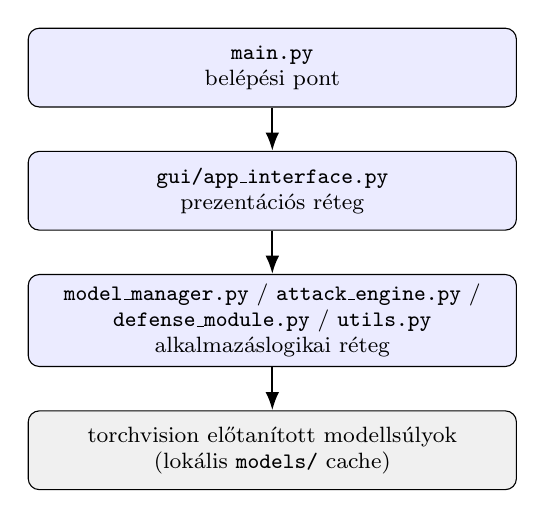
\begin{tikzpicture}[
    box/.style={draw, rounded corners, minimum width=6.2cm, minimum height=1cm,
                align=center, font=\footnotesize},
    arr/.style={-{Latex}, thick},
]
\node[box, fill=blue!8] (main) {\texttt{main.py}\\ belépési pont};
\node[box, fill=blue!8, below=0.55cm of main] (gui)
  {\texttt{gui/app\_interface.py}\\ prezentációs réteg};
\node[box, fill=blue!8, below=0.55cm of gui] (logic)
  {\texttt{model\_manager.py} / \texttt{attack\_engine.py} /\\
   \texttt{defense\_module.py} / \texttt{utils.py}\\ alkalmazáslogikai réteg};
\node[box, fill=gray!12, below=0.55cm of logic] (weights)
  {torchvision előtanított modellsúlyok\\ (lokális \texttt{models/} cache)};

\draw[arr] (main) -- (gui);
\draw[arr] (gui) -- (logic);
\draw[arr] (logic) -- (weights);
\end{tikzpicture}
\caption{A szoftver rétegei és a köztük lévő függés iránya.}
\label{fig:architecture-layers}
\end{figure}

\subsection{Az adatfolyam}
Egy tipikus támadás végrehajtása során az adat a következő lépéseken halad végig:
\begin{enumerate}
  \item A GUI a kiválasztott modellnév alapján lekéri a megfelelő \texttt{ModelBundle}-t a \texttt{ModelManager}-től,
        és ebből összeállítja az \texttt{AttackContext}-et, amely a modellt és a normalizációs paramétereket
        (átlag, szórás) fogja össze. 
  \item Az ,,Attack'' gomb megnyomásakor a GUI egy külön szálon meghívja az \texttt{attack\_engine.attack()}
        diszpécser függvényt a betöltött kép tenzorával, a kiválasztott módszerrel (FGSM vagy PGD) és paraméterekkel. 
  \item Az \texttt{attack\_engine} a kapott kontextus segítségével végrehajtja a támadást, majd egy
        \texttt{AttackResult}-ot (ellenfél alapú kép, perturbáció, tényleges iterációszám) ad vissza. 
  \item A háttérszál a főszálra ütemezve frissíti a felületet, megjeleníti az ellenfél alapú képet, a felnagyított
        perturbációt, valamint az újraszámolt predikciókat. 
  \item Amennyiben a felhasználó ezt követően védekezést is alkalmaz, a \texttt{defense\_module} az ellenfél alapú
        képre Gauss-elmosást vagy JPEG-tömörítést hajt végre, és az eredmény ugyanazon az úton kerül vissza a
        felületre. 
\end{enumerate}

Az alkalmazásnak nincs saját adatbázisa vagy perzisztens állapota. 
Az egyetlen, lemezen megmaradó adat az előtanított modellek, amelyet a \texttt{ModelManager} a
\texttt{TORCH\_HOME} környezeti változó beállításával a projekt saját \texttt{models/} könyvtárába irányít.
Ennek segítségével az adott modell csak az első használatakor töltődik le, utána a helyi cache-ből érhető el. 

\section{A felhasznált technológiák}
A szoftver Python nyelven készült, amely napjaink egyik legelterjedtebb nyelve gépi tanulási feladatokra, elsősorban a köré épült könyvtárak (PyTorch, TensorFlow, NumPy) 
ökoszisztémája miatt.

\subsubsection{Gépi tanulási keretrendszer}
Az FGSM és a PGD algoritmus egyaránt a bemeneti kép szerinti gradiensre épül, amit PyTorch deriválási mechanizmusa számol ki.
Emiatt és számos más felhasznált metódus miatt a keretrendszer választása lényegében adott volt. 
A \textbf{torchvision} biztosítja az előtanított ResNet50 és MobileNetV2 modelleket, valamint az ehhez tartozó, ImageNet-1k-n 
megszokott előfeldolgozó lépéseit (átméretezés, középre vágás, normalizálás). 
Ez az adathalmaz a képosztályozás egyik legelterjedtebb referencia-adathalmaza, ezért a legtöbb torchvision-modell is erre van előtanítva. 

\subsubsection{Grafikus felület}
A felület a \textbf{CustomTkinter} könyvtárra épül, amely a Tkinter, Python beépített GUI keretrendszerének egy modernizált rétege. 
Azért esett erre a választásom, modernebb funciókat (pl sötét témát, lekerekített gombokat és csúszkákat) ad, miközben a mögöttes eseménykezelési modell 
megegyezik a natív Tkinterével, így a Python standard könyvtárán kívül nem igényel súlyosabb GUI-függőséget. 

\subsubsection{Képfeldolgozás}
A \textbf{Pillow} könyvtár a klasszikus PIL csomag karbantartott továbbfejlesztése. 
Ez a de facto szabvány képkezelő könyvtár Pythonban, támogat minden elterjedt képformátumot támogat és jól integrálódik a NumPy/PyTorch tenzorokkal. 
Ez felelős a tenzor és a képfájl közötti átalakításokért, valamint a védekezési modul JPEG-tömörítés és Gauss-elmosás szűrőinek 
megvalósításáért. 

\subsubsection{Tesztelési eszközök}
A tesztkészlet a \textbf{pytest} keretrendszerre épül, amely a Python standard könyvtárban található \texttt{unittest}-nél tömörebb, 
függvényalapú tesztírást tesz lehetővé, illetve fixture-alapú tesztadat-előállítást és parametrizált teszteket is támogat. 
A diszpécser-függvény viselkedésének ellenőrzéséhez a \textbf{pytest-mock} könyvtár \texttt{mocker} fixture-je szükséges, amely a valódi 
implementációt burkoló (\textit{wraps}) helyettesítő objektumok (\textit{spy}) létrehozását teszi egyszerűvé. 

\subsubsection{Fejlesztői környezet}
A függőségek izolálására Python virtuális környezet (\texttt{.venv}) szolgál. 
Ez azért kell, mert a csomagok egymással kompatibilis verziói szükségesek, egy virtuális környezet biztosítja az verzióütközések elkerülését, illetve a 
működés reprodukálhatóságát. 
NVIDIA GPU esetén a PyTorch és torchvision CUDA-alapú buildje segítségével opcionálisan tovább gyorsítja mind a klasszifikációt, mind a támadások 
gradiensszámítását. 

\section{Tervezési döntések és indoklásuk}

\subsubsection{Adatstruktúrák elválasztása a funkcionális egységektől}
A kódban a modellt és a normalizációs paramétereket (\texttt{AttackContext}), a betöltött modellt
(\texttt{ModelBundle}) és egy támadás eredményét (\texttt{AttackResult}) tiszta adatstruktúrák (\texttt{dataclass}) reprezentálják, a 
műveletek pedig ezeken dolgoznak, állapot és mellékhatás nélkül. 
Ez a szétválasztás lehetővé teszi, hogy az egységtesztek a felhasználói felület és a valódi modellek mockolása nélkül fussanak. 

\subsubsection{Támadás végrehajtása háttérszálon}
Az ,,Attack'' gomb megnyomása egy \texttt{threading.Thread} példányon indítja el a támadást, mivel egy PGD-támadás már
másodperces nagyságrendű futást jelenthet, ami alatt a GUI főszál lefagyna. 

\subsubsection{FGSM interaktív epsilon-előnézet}
Egy sikeres FGSM-támadás után a felület elcache-eli a gradiens előjelét (\texttt{attack\_engine.fgsm\_sign()}), mivel az FGSM képlete ezt az
előjelet csak $\epsilon$-nal szorozza meg. 
Ezzel az $\epsilon$ csúszka mozgatásakor csak a már kiszámított előjelet kell újraskálázni, új gradienszámítás nélkül. 

\subsubsection{Modell-cache és lusta betöltés}
A \texttt{ModelManager} csak az első ténylegesen kért modellt tölti be, az eredményt egy belső cache-ben tárolja el. 
Ennek oka, hogy egy modell letöltése és felépítése másodperces nagyságrendű művelet, amit elég egyszer elvégezni. 

\subsubsection{Kiterjeszthető modellarchitektúra}
A \texttt{ModelManager.SUPPORTED} lista és a \texttt{\_build()} metódus egyetlen helyen tartja a rendelkezésre álló modelleket, így egy új
torchvision-modell integrálása más kód módosítása nélkül megoldható. 

\subsubsection{A bemeneti kép 224×224-es mérete}
A betöltött kép mérete előbb $256$ pixelre kerül átméretezésre, majd $224\times224$-re középre vágásra (\texttt{Resize(256)} + \texttt{CenterCrop(224)}), mivel
mind a ResNet50, mind a MobileNetV2 erre a méretre lett előtanítva. 
Erre azért van szükség, mert a nyers képek aránya általában nem négyzetes, egy közvetlen $224\times224$-re történő átméretezés vizuálisan eltorzítaná a képet. 
Emiatt viszont a kép szélén lévő tartalom elveszhet. 
Azt az elvárt felhasználói esetet, hogy a támadott képet visszatöltve ugyanazt az osztályozást kapjuk, az átméretezés és a vágás pontosan $224\times224$ méretű képre elmarad. 

\section{Az egyes komponensek megvalósítási részletei}
A megvalósítási részletek alatt nem célom felfedni az egész program belső működését, csak bemutatok pár érdekesebb részletet és példának az fgsm 
metódus teljes kódját. 

\subsection{\texttt{model\_manager.py} modul}
\begin{itemize}
  \item A \texttt{ModelBundle} a betöltött hálón (\texttt{model}) kívül az ImageNet-1k normalizációs átlagot és szórást is $(1, 3, 1, 1)$ alakú
        tenzorként tárolja, hogy a támadás során a csatornánkénti normalizálás egyetlen elemenkénti művelettel elvégezhető legyen
        tetszőleges méretű bemeneti képen. 
  \item A betöltés után a modell minden paraméterén explicit módon \texttt{requires\_grad\_(False)} hívás történik, mivel a támadáshoz kizárólag a bemeneti
        kép szerinti gradiens ($\nabla_x J$) szükséges, a modell súlyai szerinti gradienst sosem számoljuk ki. 
  \item Ha az eszköz nem explicit adott, akkor a konstruktor \texttt{"cuda"}-t választ, amennyiben elérhető CUDA-képes GPU 
        (\texttt{torch.cuda.is\_available()}), egyébként \texttt{"cpu"} lesz az érték. 
\end{itemize}

\subsection{\texttt{attack\_engine.py} modul}
Először összeállítja a támadást aszerint, hogy melyik algoritmus szükséges és hogy célzott-e a támadás. 
Ezután hívja meg a tényleges \texttt{\_fgsm} vagy \texttt{\_pgd} implementációt, végül az eredményt egységesen egy \texttt{AttackResult}-ba
csomagolja. 
A \ref{lst:fgsm}. kódrészlet az FGSM implementációját mutatja. 

\begin{lstlisting}[language=Python, caption={Az FGSM implementációja (\texttt{attack\_engine.\_fgsm})}, label={lst:fgsm}]
def _fgsm(ctx, x, y, epsilon, targeted):
    x_adv = x.clone().detach().requires_grad_(True)
    unnormalized_scores = _forward(ctx, x_adv)
    loss = F.cross_entropy(unnormalized_scores, y)

    grad = torch.autograd.grad(loss, x_adv)[0]
    sign = grad.sign()
    if targeted:
        x_adv = x_adv - epsilon * sign
    else:
        x_adv = x_adv + epsilon * sign

    x_adv = torch.clamp(x_adv, 0.0, 1.0)
    return x_adv.detach()
\end{lstlisting}

A metódusban mindenek előtt a bemeneti kép tenzorát a \texttt{detach()} hívással leválasztjuk a számítási gráfról, majd a
\texttt{requires\_grad\_(True)} hívás a tenzort a gráf új levelévé teszi és bekapcsolja rá a gradienskövetést, hogy a következő forward lépés
után a bemeneti kép szerint is deriválható legyen. 
A \texttt{torch.autograd.grad} hívás a veszteség bemeneti kép szerinti gradiensét adja vissza egyetlen hátrafelé irányuló lépésben, ez a korábban használt 
jelölés szerinti $\nabla_x J(\theta, x, y)$-t. 
Ezután a célzott és normál támadás közti elágazás következik, ahol a kifejezés csak egy előjelben különbözik. 
A visszatérési értéket a \texttt{clamp} alkalmazásával szorítjuk vissza az $[0, 1]$ pixeltartományra, majd a végén egy \texttt{detach()} hívás
biztosítja, hogy a visszaadott tenzor ne hordozzon további autograd-gráf hivatkozást. 

\subsection{\texttt{defense\_module.py} modul}
A védekezés PIL-alapú műveletekből áll, ezért a modul minden hívás előtt és után elvégez egy, a pixeltér-tenzor és a PIL kép közötti konverziót. 
\begin{itemize}
  \item A JPEG-tömörítés egy memóriában tartott bájtpuffert (\texttt{io.BytesIO}) használ, ebbe kódolja be a képet a megadott minőséggel, majd
        ugyaninnen dekódolja azt vissza. Tehát nem történik lemezre írás, így ténylegesen egy veszteséges tömörítés-visszafejtés történik, nem csak
        annak szimulációja. 
  \item A Gauss-elmosás a PIL \texttt{ImageFilter.GaussianBlur} szűrőjét alkalmazza a megadott sugárral. 
\end{itemize}

\subsection{\texttt{utils.py} modul}
A nyers $\delta$ perturbáció felhasználói felületen ábrázolásához pár részlet. 
Mivel értékei jellemzően nagyon kis abszolút értékűek, ennek megjelenítése gyakorlatilag egyszínű,
szemmel kivehetetlen képet adna. 
A \texttt{perturbation\_to\_pil} függvény ezért a perturbációt egy \texttt{magnify} szorzóval felnagyítja, majd $0{,}5$-tel eltolja, mielőtt a
$[0, 1]$ tartományra vágná. 
Az eltolás azért szükséges, hogy ábrázoljuk a negatív előjelű változást, különben azok a $[0, 1]$ tartományra vágásnál elvesznének. 
Az eltolás miatt egy nulla közeli (gyakorlatilag változatlan) pixel középszürkeként jelenik meg, míg a pozitív és negatív irányú változások
világosabb, illetve sötétebb árnyalatként válnak láthatóvá. 

\chapter{Tesztelés}

\section{Egységtesztek}
A program tesztkészletének felépítésénél a szakirodalomból ismert \textit{tesztpiramisnak} nevezett
hierarchiát követtem~\cite{fowler2012testpyramid}. Ennek alapját a gyorsabb és kevés komponenst érintő tesztek, az egységtesztek képezik, 
melyek a lehető legkisebb elkülöníthető egységek tesztelését valósítják meg. Futási idejük 
jellemzően ezredmásodperces tartományban mozog és akár lefedhetik az input paraméterek teljes értékkészletét. Az elkészítésüknél fontos szempont a 
többi egységtől való függetlenség (izoláció) és az perifériáktól való függetlenség, I/O, adatbázis, hálózat, stb. Ezeknek a teszteknek az elkészítésére 
érdemes nagy figyelmet fordítani, mivel a korai szakaszban feltárt hibák javítása általában lényegesen olcsóbb, mint a később, integráció vagy éles 
környezetben felfedezetteké.

Az egységtesztek tudatosan nem a valódi, előtanított ResNet50/MobileNetV2 modelleket használják. Az
\texttt{attack\_engine} teszteknél egy \texttt{tiny\_model} fixture ad egy $5$ osztályos,
$8\times8$ pixeles bemenetet feldolgozó, egyetlen lineáris rétegből álló hálót. Ez a döntés a tesztek sebességét 
(a valódi háló letöltése és felépítése másodperces nagyságrendű lenne) és izoláltságát szolgálja: a teszt kizárólag a 
saját kódunk logikáját vizsgálja, nem a harmadik féltől származó architektúra pontosságát. 

Minden véletlent felhasználó fixture (pl. a bemeneti képet generáló \texttt{sample\_image\_tensor})
maga hívja meg a \texttt{torch.manual\_seed}-et közvetlenül az adat előállítása előtt, így a
determinizmus független a fixture-ök végrehajtási sorrendjétől. Az egységtesztek szintjén nem támadási sikerrátát mérünk (ehhez sok mintás, statisztikai kiértékelés
kellene), hanem az algoritmusok tulajdonságait ellenőrizzük
konkrét, kis méretű bemeneteken.

Ebben a részben a számosságuk miatt nem mutatom be az összes egységtesztet, csak a középpontban álló \texttt{attack\_engine.py} 
modult mivel ez valósítja meg az alkalmazás lényegi logikáját (az FGSM és PGD algoritmusokat,
valamint az ezeket kiszolgáló \texttt{predict()} és \texttt{attack()} függvényeket). 

\bigskip
\noindent\textbf{A \texttt{predict()} és a diszpécser (\texttt{attack()}) tesztjei}

\medskip
\noindent\texttt{test\_predict\_re\-turns\_topk\_shapes}: Ellenőrzi, hogy \texttt{topk=3} esetén a visszaadott
valószínűség- és index-tenzor alakja $(1, 3)$, azaz a batch- és $k$-dimenzió megfelel a kérésnek.

\medskip
\noindent\rule{\linewidth}{0.3pt}

\medskip
\noindent\texttt{test\_predict\_re\-turns\_valid\_distribution}: A \texttt{topk=5} valószínűségek mindegyike a
$[0, 1]$ intervallumba esik, és -- mivel az 5 osztályos \texttt{tiny\_model} minden osztálya lekérdezésre
kerül -- összegük $1{,}0$-ra \texttt{allclose}. Ez a softmax kimenet valódi valószínűségi eloszlás voltát
igazolja.

\medskip
\noindent\rule{\linewidth}{0.3pt}

\medskip
\noindent\texttt{test\_predict\_top\-k\_returns\_highest\_first}: A visszaadott valószínűségek csökkenő
sorrendben szerepelnek ($\mathrm{probs}[0, i] \geq \mathrm{probs}[0, i+1]$), vagyis a \texttt{topk} valóban a
legnagyobb konfidenciájú osztályokat adja vissza, méghozzá rendezetten.

\medskip
\noindent\rule{\linewidth}{0.3pt}

\medskip
\noindent\texttt{test\_attack\_unk\-nown\_method\_raises}: Határeset: egy nem létező módszernév
(\texttt{"NEM VALID"}) megadásakor \texttt{ValueError}-t vár, mielőtt bármilyen gradiensszámítás történne --
a bemenet-validáció a drága számítás előtt fut le.

\medskip
\noindent\rule{\linewidth}{0.3pt}

\medskip
\noindent\texttt{test\_attack\_fgsm\_ig\-nores\_iterations\_argument}: Annak ellenére, hogy a hívó
\texttt{iterations=99}-et ad át, FGSM esetén a visszaadott \texttt{AttackResult.iterations\_run} értéke $1$ --
igazolva, hogy az FGSM valóban egylépéses, és a paramétert a diszpécser figyelmen kívül hagyja erre a
módszerre.

\medskip
\noindent\rule{\linewidth}{0.3pt}

\medskip
\noindent\texttt{test\_attack\_pgd\_re\-ports\_requested\_iteration\_count}: PGD esetén a kért iterációszám
($4$) változatlanul megjelenik az \texttt{iterations\_run} mezőben, alátámasztva, hogy a diszpécser a
paramétert továbbadja a \texttt{\_pgd} implementációnak.

\medskip
\noindent\rule{\linewidth}{0.3pt}

\medskip
\noindent\texttt{test\_attack\_fgsm\_dis\-patches\_only\_to\_fgsm}: \texttt{mocker.patch(..., wraps=\_fgsm)} és
\texttt{wraps=\_pgd} spy-okkal figyeli a hívásokat: \texttt{method="FGSM"} esetén
\texttt{\_fgsm.assert\_called\_once()} és \texttt{\_pgd.assert\_not\_called()} teljesül. A \texttt{wraps}
paraméter miatt a valódi implementáció is lefut, tehát az \texttt{AttackResult} összeállítása is ellenőrzött
marad.

\medskip
\noindent\rule{\linewidth}{0.3pt}

\medskip
\noindent\texttt{test\_attack\_pgd\_dis\-patches\_only\_to\_pgd}: Az előző teszt tükörképe:
\texttt{method="PGD"} esetén kizárólag \texttt{\_pgd} hívódik meg, \texttt{\_fgsm} nem. A két teszt együtt
zárja ki, hogy a diszpécser valamelyik ágon ,,átcsorogva'' mindkét algoritmust lefuttassa.

\bigskip
\noindent\textbf{Az FGSM implementáció (\texttt{\_fgsm}) tesztjei}

\medskip
\noindent\texttt{test\_fgsm\_targeted\_steps\_opposite\_direction\_of\_untargeted}: Azonos bemeneten és
$\epsilon$ mellett a célzott és nem célzott perturbáció pontosan ellentétes előjelű
($x_{\text{nem célzott}} - x = -(x_{\text{célzott}} - x)$), ami közvetlenül a matematikai definícióból (a
gradiens előjelének megfordításából) következik.

\medskip
\noindent\rule{\linewidth}{0.3pt}

\medskip
\noindent\texttt{test\_fgsm\_clamps\_to\_valid\_pixel\_range}: Szélsőséges bemenet (csupa nulla pixel) és
nagy $\epsilon=0{,}5$ mellett is a kimenet minden eleme a $[0, 1]$ tartományban marad -- igazolva, hogy a
\texttt{clamp} lépés ténylegesen érvényesül, nem csak elméletben szerepel a specifikációban.

\medskip
\noindent\rule{\linewidth}{0.3pt}

\medskip
\noindent\texttt{test\_fgsm\_re\-sult\_is\_de\-tached\_from\_autograd}: A visszaadott tenzor
\texttt{requires\_grad} attribútuma \texttt{False}.

\medskip
\noindent\rule{\linewidth}{0.3pt}

\medskip
\noindent\texttt{test\_fgsm\_re\-sult\_has\_no\_graph\_history}: Szigorúbb bizonyíték az előzőnél:
\texttt{grad\_fn is None} \emph{és} \texttt{is\_leaf is True} egyszerre teljesül, ami kizárja azt az esetet
is, amikor egy tenzor \texttt{requires\_grad} értéke hamis, de mégis egy számítási gráf levele marad rejtett
hivatkozásokkal.

\medskip
\noindent\rule{\linewidth}{0.3pt}

\medskip
\noindent\texttt{test\_fgsm\_ze\-ro\_epsi\-lon\_re\-turns\_original}: Határeset: $\epsilon=0$ esetén a perturbáció
nulla, a kimenet \texttt{allclose} az eredeti képpel -- az algoritmus degenerált esetben identitásként
viselkedik.

\medskip
\noindent\rule{\linewidth}{0.3pt}

\medskip
\noindent\texttt{test\_fgsm\_un\-targeted\_re\-duces\_confidence\_in\_true\_label}: Viselkedési bizonyíték: a
\texttt{predict()}-en keresztül lekérdezett, a valódi címkéhez tartozó konfidencia a támadás \emph{után}
szigorúan kisebb, mint előtte -- ez nem csak a perturbáció létezését, hanem annak tényleges hatását igazolja
a modell kimenetére.

\medskip
\noindent\rule{\linewidth}{0.3pt}

\medskip
\noindent\texttt{test\_fgsm\_tar\-geted\_in\-creases\_confidence\_in\_target\_label}: A célzott változat
tükörpárja: a mesterségesen kiválasztott célosztály konfidenciája nő a támadás hatására, alátámasztva, hogy a
célzott mód valóban a célosztály felé tereli a predikciót, nem csupán ,,valamerre'' téveszti meg a modellt.

\bigskip
\noindent\textbf{A PGD implementáció (\texttt{\_pgd}) tesztjei}

\medskip
\noindent\texttt{test\_pgd\_re\-sult\_stays\_within\_epsilon\_ball}: Mérsékelt lépésméret ($\alpha=0{,}02$)
mellett a végső perturbáció minden pixelre $|\delta| \leq \epsilon + 10^{-6}$ (a tolerancia a lebegőpontos
kerekítést kompenzálja) -- ez az $\ell_\infty$-gömbbe való projekció alapvető helyességét igazolja.

\medskip
\noindent\rule{\linewidth}{0.3pt}

\medskip
\noindent\texttt{test\_pgd\_hits\_ball\_when\_step\_too\_large}: Szándékosan irreálisan nagy lépésméretet
($\alpha=10{,}0 \gg \epsilon=0{,}02$) ad meg, ami minden iterációban túllövést okoz; ilyenkor a projekciós
\texttt{clamp}-nek kell egyedül biztosítania a korlátot, ezért a tesztben a végső $|\delta|$ pontosan (nem
csak $\leq$) $\epsilon$-nak adódik minden pixelen -- ez a projekció, nem a lépésméret helyes megválasztása
általi korlátozottságot bizonyítja.

\medskip
\noindent\rule{\linewidth}{0.3pt}

\medskip
\noindent\texttt{test\_pgd\_clamps\_to\_valid\_pixel\_range}: A pixeltartomány-korlátozás ugyanúgy teljesül
PGD esetén is, mint FGSM-nél: szélsőséges (nulla) bemeneten és nagy $\epsilon$ mellett a kimenet a $[0, 1]$
tartományban marad.

\medskip
\noindent\rule{\linewidth}{0.3pt}

\medskip
\noindent\texttt{test\_pgd\_re\-sult\_has\_no\_graph\_history}: Ugyanaz az erős \texttt{detach}-bizonyíték
(\texttt{grad\_fn is None} és \texttt{is\_leaf is True}), mint FGSM esetén -- fontos, mert a PGD több
iterációt is végez, minden lépésben új \texttt{requires\_grad\_(True)} hívással, így könnyebben
,,elszivároghatna'' egy hivatkozás a gráfra, ha a ciklus végén elmaradna a leválasztás.

\medskip
\noindent\rule{\linewidth}{0.3pt}

\medskip
\noindent\texttt{test\_pgd\_ze\-ro\_epsi\-lon\_re\-turns\_original}: Határeset: $\epsilon=0$ esetén -- annak
ellenére, hogy több iteráció is lefut -- a projekció minden lépésben nulla szélességű intervallumra
szorítja a perturbációt, így a végeredmény megegyezik az eredeti képpel.

\medskip
\noindent\rule{\linewidth}{0.3pt}

\medskip
\noindent\texttt{test\_pgd\_un\-targeted\_re\-duces\_confidence\_in\_true\_label}: Viselkedési bizonyíték
\texttt{predict()}-en keresztül: a valódi címke konfidenciája több iteráció után is csökken -- ugyanaz az
elv, mint FGSM-nél, de itt azt is igazolja, hogy az iteratív frissítés nem ,,rontja el'' a kumulatív hatást.

\medskip
\noindent\rule{\linewidth}{0.3pt}

\medskip
\noindent\texttt{test\_pgd\_tar\-geted\_in\-creases\_confidence\_in\_target\_label}: A célzott PGD a célosztály
konfidenciáját növeli -- ugyanazon tulajdonságpár (nem célzott csökkenti/célzott növeli a releváns
konfidenciát) FGSM-re és PGD-re is parametrizált formában lett tesztelve
(\texttt{@pytest.mark.parametrize}), elkerülve, hogy csak az egyik algoritmusra íródjon le a viselkedés.

\bigskip

\section{Integrációs tesztek}

Az integrációs tesztek a képbetöltő, a modellkezelő és a támadómotor együttműködését ellenőrzik. 
A \texttt{test\_image\_loading\_and\_attack} teszt az FGSM és a PGD módszert is ellenőrzi. 
A modellkezelőben a MobileNetV2 hálót egy kis méretű tesztmodell helyettesíti, de a képbetöltés, a modellkezelés és a támadás mockolás nélkül fut. 
Továbbá a teszt ellenőrzi, hogy a támadás megváltoztatja a képet, az eredmény $\epsilon$ korláton és az érvényes pixeltartományon belül marad, illetve osztályozható. 

A \texttt{test\_cached\_mobilenet\_pgd} teszt ugyanezeknek a moduloknak az együttműködését az előtanított MobileNetV2 modellen vizsgálja. 
Hogy mindenképp gyors legyen, a teszt csak akkor fut le, ha a modell súlyai már megtalálhatók a helyi gyorsítótárban. 


\section{Automatizált GUI tesztek}

A grafikus felület ellenőrzésére öt automatizált tesztet készítettem. 
Ezek a CustomTkinter valódi felületi elemeit hozzák létre, majd a gombok programozott interakcióival vizsgálják a felület reakcióját. 
Az ablak a tesztek idejére rejtett, de a futtatáshoz szükséges a grafikus környezet. 
Az élesben használt modellek helyett kis tesztmodell működik, így nincs szükség súlyok letöltésére, tehát a teszt gyors marad.

\bigskip
\noindent\textbf{A felület kezdeti állapota}

\medskip
\noindent A \texttt{test\_initial\_state} ellenőrzi, hogy induláskor nincs betöltött eredeti vagy támadott kép, a képmezők üresek, és az alapértelmezett támadási módszer az FGSM. 

\medskip
\noindent A \texttt{test\_attack\_without\_image\_shows\_message} az \texttt{Attack} gombot kép betöltése nélkül hívja meg. 
Ellenőrzi, hogy a felület a megfelelő tájékoztató üzenetet kéri, és nem indít támadási szálat. 

\bigskip
\noindent\textbf{Kép betöltése és célosztály kiválasztása}

\medskip
\noindent A \texttt{test\_load\_image\_updates\_display\_and\_predictions} a \texttt{Load Image} gombbal egy tesztképet tölt be. 
Ellenőrzi a betöltött tenzor méretét, a képmező és a három predikció frissülését, valamint a státuszüzenetet. 

\medskip
\noindent A \texttt{test\_select\_target\_updates\_checkbox\_and\_status} a szűrt célosztálylistából kiválaszt egy osztályt. 
Ellenőrzi a kiválasztott osztályt, a célzott támadás jelölőnégyzetének állapotát és a státuszüzenetet. 

\bigskip
\noindent\textbf{Támadás és alaphelyzetbe állítás}

\medskip
\noindent A \texttt{test\_attack\_then\_reset\_updates\_images} egy betöltött képen elindítja az FGSM támadást. 
Ellenőrzi, hogy megjelenik a perturbáció és a támadott kép, frissülnek a predikciók, és a státuszsor jelzi a támadás végét. 
Ezután a \texttt{Reset} gomb hatására a támadott kép és predikciói törlődnek, míg az eredeti kép és predikciói megmaradnak. 

\section{Funkcionális tesztek és felhasználói validáció}

A grafikus felület funkcionális, ,,fekete doboz'' teszteseteit a felhasználói forgatókönyvek alapján,
\textit{Given--When--Then} formában fogalmazom meg. Az alábbi esetek a tényleges
felhasználói felületének elemeihez (gombok, csúszkák, célosztály-kereső) igazodnak, és kézi
(manuális) végrehajtásra tervezettek.

\begin{itemize}
  \item \textbf{Kép betöltése a ,,Load Image'' gombbal}\\
    AS A: felhasználó \textsc{I want to}: egy képet betölteni a vizsgálathoz\\
    \textsc{Given}: az alkalmazás elindítva, még nincs kép betöltve\\
    \textsc{When}: a ,,Load Image'' gombra kattint, majd egy érvényes képfájlt választ ki\\
    \textsc{Then}: az ,,Original'' képmezőben megjelenik a beolvasott, $224\times224$-re vágott
      kép, és alatta a top-3 predikció és konfidencia frissül

  \item \textbf{Modell váltása betöltött kép mellett}\\
    AS A: felhasználó \textsc{I want to}: összehasonlítani, hogy más architektúra hogyan látja a képet\\
    \textsc{Given}: egy kép már be van töltve, az ,,Original'' predikciós panel ki van töltve\\
    \textsc{When}: a modell-választó legördülőben ,,MobileNetV2''-t választ ,,ResNet50'' helyett\\
    \textsc{Then}: az ,,Original'' predikciók újraszámolódnak az új modellel; ha korábban már
      futott támadás, az ,,Adversarial'' predikciók is frissülnek

  \item \textbf{Nem célzott támadás végrehajtása}\\
    AS A: felhasználó \textsc{I want to}: általános tévesztést előidézni a modellben\\
    \textsc{Given}: kép betöltve, ,,Targeted attack'' jelölőnégyzet kikapcsolva, $\epsilon$ és
      iterációszám csúszkák beállítva\\
    \textsc{When}: az ,,Attack'' gombra kattint\\
    \textsc{Then}: a státuszsor ,,Running...'' majd ,,Attack complete'' üzenetet mutat, megjelenik
      a felnagyított perturbáció és a támadott kép, és az ,,Adversarial'' predikciós panelen az
      eredeti top-1 osztály konfidenciája jellemzően csökken

  \item \textbf{Célzott támadás célosztály kereséssel}\\
    AS A: felhasználó \textsc{I want to}: egy konkrét osztályra rávenni a modellt\\
    \textsc{Given}: kép betöltve, a célosztály-kereső mezőbe elkezd gépelni egy osztálynevet\\
    \textsc{When}: a szűrt listából kiválaszt egy osztályt, majd az ,,Attack'' gombra kattint\\
    \textsc{Then}: a ,,Targeted attack'' jelölőnégyzet automatikusan bejelölődik, a státuszsor a
      kiválasztott osztály nevét mutatja, és a támadás után a célosztály konfidenciája nő

  \item \textbf{Epsilon csúszka élő előnézete FGSM módban}\\
    AS A: felhasználó \textsc{I want to}: interaktívan látni, hogyan változik a perturbáció
      erőssége\\
    \textsc{Given}: FGSM módszerrel már lefutott egy támadás (a gradiens előjele cache-elve van)\\
    \textsc{When}: az $\epsilon$ csúszkát új értékre húzza, PGD-re váltás nélkül\\
    \textsc{Then}: a perturbáció és az ellenfél alapú kép új gradiens-számítás \emph{nélkül},
      azonnal újraszámolódik a cache-elt előjel alapján

  \item \textbf{Attack gomb kép nélkül}\\
    AS A: felhasználó \textsc{I want to}: (véletlenül) támadást indítani kép betöltése előtt\\
    \textsc{Given}: az alkalmazás elindítva, nincs betöltött kép\\
    \textsc{When}: az ,,Attack'' gombra kattint\\
    \textsc{Then}: egy ,,No image'' információs párbeszédablak jelenik meg, a támadás nem indul el

  \item \textbf{Védekezési szűrő alkalmazása (Blur / JPEG)}\\
    AS A: felhasználó \textsc{I want to}: megvizsgálni, hogy egy egyszerű szűrő semlegesíti-e a
      zajt\\
    \textsc{Given}: egy sikeres támadás után az ,,Adversarial'' kép elérhető\\
    \textsc{When}: a ,,Defend (Blur)'' vagy ,,Defend (JPEG)'' gombra kattint\\
    \textsc{Then}: az ,,Adversarial'' képmező a szűrt képre frissül, és a predikciós panel az
      újraosztályozott (a szűrés után kapott) eredményeket mutatja

  \item \textbf{Defend gomb ellenfél alapú kép nélkül}\\
    AS A: felhasználó \textsc{I want to}: (véletlenül) védekezést alkalmazni támadás előtt\\
    \textsc{Given}: kép be van töltve, de még nem futott támadás\\
    \textsc{When}: valamelyik ,,Defend'' gombra kattint\\
    \textsc{Then}: egy ,,No adversarial'' információs párbeszédablak jelenik meg, semmilyen kép
      nem változik

  \item \textbf{Az eredeti kép letöltése}\\
    AS A: felhasználó \textsc{I want to}: az eredeti képet fájlba menteni\\
    \textsc{Given}: egy kép be van töltve\\
    \textsc{When}: a ,,Download original'' gombra kattint\\
    \textsc{Then}: mekapja a mentett $224\times224$ pixeles fájlt

  \item \textbf{A támadott kép letöltése és visszatöltése}\\
    AS A: felhasználó \textsc{I want to}: az ellenfél alapú képet elmenteni és újra feltölteni\\
    \textsc{Given}: egy sikeres támadás után az ,,Adversarial'' kép létrejön\\
    \textsc{When}: a ,,Download adversarial'' gombra kattint, elmenti PNG-ben, majd a ,,Load Image'' gombbal visszatölti\\
    \textsc{Then}: a visszatöltött kép ugyanazt a top-1 osztályozást adja, a konfidencia pedig csak minimálisan tér el

  \item \textbf{Letöltés kép vagy támadás nélkül}\\
    AS A: felhasználó \textsc{I want to}: (véletlenül) letöltést kérni, mielőtt volna mit menteni\\
    \textsc{Given}: nincs betöltött kép, illetve van kép, de még nem futott támadás\\
    \textsc{When}: a ,,Download original'' vagy a ,,Download adversarial'' gombra kattint\\
    \textsc{Then}: egy ,,No image'' vagy ,,No adversarial'' információs párbeszédablak jelenik meg, fájl nem készül

  \item \textbf{Reset gomb}\\
    AS A: felhasználó \textsc{I want to}: új kísérletet kezdeni ugyanazzal a képpel\\
    \textsc{Given}: egy támadás és esetleg egy védekezés már lefutott\\
    \textsc{When}: a ,,Reset'' gombra kattint\\
    \textsc{Then}: a perturbáció és az ,,Adversarial'' képmező üresre vált, az ,,Adversarial''
      predikciós panel névtelen (,,---'') állapotba áll vissza, az ,,Original'' kép és predikciói
      változatlanok maradnak

  \item \textbf{Hibakezelés támadás közben}\\
    AS A: felhasználó \textsc{I want to}: érthető visszajelzést kapni, ha a támadás valamiért
      meghiúsul\\
    \textsc{Given}: kép betöltve, a háttérszálon futó \texttt{\_attack\_worker} kivételt dob (pl.
      eszközhiba miatt)\\
    \textsc{When}: az ,,Attack'' gombra kattint\\
    \textsc{Then}: egy ,,Attack failed'' hibaablak jelenik meg a teljes veremkiíratással, a
      státuszsor ,,Attack failed.'' szöveget mutat, az alkalmazás nem fagy le
\end{itemize}

\section{Teszteredmények és értelmezésük}

A \ref{fig:tesztfuttatas}. ábra a teljes teszt csomag futtatásának eredményét mutatja. 
A futtatás a $76$ teszt sikeresen lefutott, köztük $68$ egységteszt, $3$ integrációs teszt és $5$ grafikus felületi teszt. 
Az eredmény a vizsgált esetek sikerességét mutatja, ám önmagában nem igazolja a program teljes hibamentességét. 

\begin{figure}[htb]
\centering
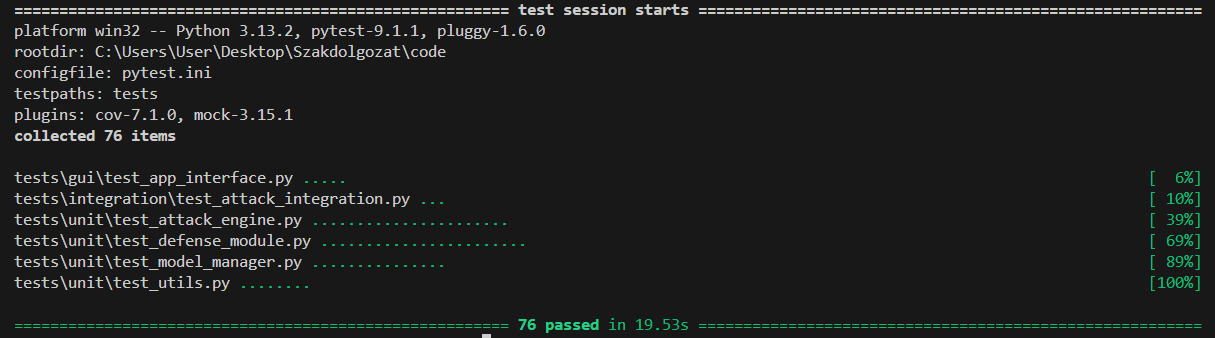
\includegraphics[width=\linewidth]{images/test_run.PNG}
\caption{Az automatizált tesztek sikeres futtatásának kimenete}
\label{fig:tesztfuttatas}
\end{figure}

\section{A tesztelés korlátai}

Az automatizált tesztek néhány kiválasztott bemeneten ellenőrzik a szoftver működésének egyes tulajdonságait, de nem garantálják a szoftver hibamentességét. 
A modellt igénylő tesztek többségében a gyorsaság és a megismételhetőség érdekében kisméretű tesztmodellt használunk. 
Egyetlen integrációs teszt használja az előtanított MobileNetV2 hálót, ez a teszt a modell súlyainak hiányában kimarad. 
A tesztekben felhasznált bemenetek között véletlenszerűen előállított tenzorok és egyszínű tesztképek szerepelnek. 
Ezek alkalmasak a működés egyes tulajdonságainak ellenőrzésére, de nem elegendők ahhoz, hogy általános következtetéseket vonjunk le a modellek vagy a támadások sikerességéről. 

A grafikus felület tesztjei valódi felületi elemeket hoznak létre, de a gombokat programozottan hívják meg, nem felhasználói interakcióval. 
A támadást ellenőrző tesztben a munkafüggvény nem külön háttérszálon fut, így a teszt nem vizsgálja a párhuzamos futásból eredő eseteket. 
A tesztek nem fedik le a felület minden funkcióját, és a megjelenés vizuális helyességét sem ellenőrzik. 

\chapter{Összefoglalás}

\section{Elért eredmények}

\section{Következtetések}

\section{Továbbfejlesztési lehetőségek}
\cleardoublepage

\nocite{dziugaite2016jpeg}
\phantomsection
\addcontentsline{toc}{chapter}{\biblabel}
\printbibliography[title=\biblabel]
\cleardoublepage

\end{document}
